\chapter{Hydrogen Bond Dynamics of Water/Vapor Interfaces }\label{CHAPTER_HB}
There are two types of bonds in water: the stronger covalent bonds (molecular $\sigma$ bonds) within a single water molecule and 
the much weaker H-bonds between water molecules.
H-bonds play a critical role in the behaviour of bulk water,\cite{Eisenberg1969,Luzar1996,Cabane2005} water near interfaces,\cite{Chowdhary2008} 
and aqueous solutions. \cite{Naslund2005} There are many methods to study the hydrogen bond (HB) dynamics in water, solutions or interfaces, 
such as molecular dynamics simulation,\cite{Chowdhary2008,Banerjee2016}, neutron scattering, etc.
In this chapter, we will introduce the general concepts and methods of HB Dynamics (HBD)\cite{AL96,Luzar1996,DC87} used to analyze the structure 
and dynamic properties of bulk solutions and gas-liquid interfaces. 

\section{Definitions of Hydrogen Bond Population and Correlation Functions}
Luzar and Chandler [\cite{AL96}] have elucidated the HB dynamics of pure water, and
subsequently such analysis has been also extended to explore the HB dynamics
in complex situations, e.g., electrolytes, [\cite{AC00}] protein and  micellar surfaces. [\cite{SP05}]
There are temporal, geometric and energetic criteria to define HB. Here we use the geometric one.
Two water molecules are H-bonded only if their interoxygen distance between of specific tagged pair of water molecules 
is less than $r^{\text{c}}_{\text{OO}}$ and
the O-H$\cdots$O angle is less than $\phi^{\text{c}}$. [\cite{AKS86,JT90,SB02}] 
The value $r^{\text{c}}_{\text{OO}}$ corresponds to the first-minimum position of the O--O RDF of water. [\cite{Sciortino1989}]   
The choice for the cutoff angle $\phi^{\text{c}}$ for water-water molecules is obtained by studying the average number of H-bonds,
as a function of $\phi^{\text{c}}$. \cite{Luzar1993} We call this definition of HB the ADH criterion. 
In order to compare the impact of different HB definitions on HB dynamics, we will also use another definition of HB in our analysis. 
When the distance between the oxygen atoms of two water molecules is less than $r^{\text{c}}_{\text{OO}}$, 
and the oxygen-hydrogen-oxygen included angle is greater than a critical angle $\theta^{\text{c}}$, then we say that there is a HB between the two molecules. 
We denote this definition as the AHD definition of H bonds.
%The distance criteria of $R_{\text{OH}}$  was determined from the first minimum in the O--H RDF for SPC water. [\cite{HJCB81}]

% introduce h(t)
The configuration criterion above allows us to define a variable $h[r(t)] = h(t)$, HB population. 
The $h(t)$ has a value 1 when the particular tagged pair of molecules are bonded, and 0 otherwise. 
%=================
% added 2020-5-27: to show that h(t) is actually the fluctuation of itself (\delta h).
We know that the instantaneous fluctuation or deviation in a dynamical variable $A(t)$ from its time-independent equilibrium average $\langle A\rangle$ , 
is defined by [\cite{DC87}] 
$$
\delta A = A(t) - \langle A\rangle.
$$
For the $h(t)$, since the probability that a specific pair of molecules is bonded in a large system is extremely small, i.e., 
the time average of $h$ is zero, or  
$\langle h \rangle = 0$,
then
$$
\delta h(t) = h(t).
$$
Therefore, the $h(t)$ describe the instantaneous fluctuation $\delta h(t)$  of the HB population.  
%The behaviour of $r_{OO}(t)$  is depicted in Fig.\ref{fig:Ex30ps_hb}(a). We find that in the equilibrium system, $r_{OO}(t)$ looks chaotic.
%=================

While the equilibrium average of the $\delta h(t)$ is zero, but we can obtain useful information by considering the equilibrium 
correlations between fluctuations at different times. The correlation between the $\delta h(t)$ and the $\delta h(0)$ can be written as 
$$
\langle \delta h(0) \delta h(t)\rangle = \langle h(0)h(t)\rangle-\langle h \rangle^2 = \langle h(0)h(t)\rangle,
$$
where the averaging $\langle\cdots\rangle$ is to be performed over the ensemble of initial conditions $(r^N, p^N)$.


In this section, we will use three correlation functions to describe the HB dynamics of water/vapor interfaces of solutions,
the HB population correlation function \CHB, the survival probability \SHB and the reactive flux $k(t)$. [\cite{Rapaport1983}]

\paragraph{Structure of HB Network}
One of the importrant characteristics of HB network is the average number of H-bonds per molecule. 
At room temperature and atmospheric pressure, this quantity is close to four or slightly higher. \cite{Malenkov2006} 

Furthermore, one can consider a more detailed distribution function. A molecule can form multiple H-bonds with other molecules at the same time.
 Among these H-bonds, the molecule has $i$ times in the form of donors and $j$ times in the form of acceptors, 
that is, the total number of H-bonds formed by the molecule at a certain time is $i+j$.
Regarding the H-bonding of pure bulk water, people have obtained rich results with this analysis method and MD simulations. \cite{Malenkov1990,Malenkov2006}

\paragraph{HB Population Auto-Correlation Function}
We use the correlation function \CHB to describe the structural relaxation of H-bonds: 
\begin{eqnarray}
C_{\text{HB}}(t)=\langle h(0)h(t) \rangle/\langle h\rangle
\label{eq:C_HB}.
\end{eqnarray}
With the aid of the ergodic principle, the ensemble average $\langle \cdots\rangle$ is implemented by time average.
The $\langle h\rangle$ is the probability that a pair of randomly chosen water molecules in the system is
H-bonded in a certain form at any time $t$. 
Here is an explanation of the specific meaning of the word "form". 
Each water molecule has two H atoms and one O atom. Therefore, when a pair of water molecules $a$ and $b$ are bonded by a H-bond, 
the oxygen atom in each water molecule can act as both a donor and an acceptor. When water molecules $a$ and $b$ are used as donors, 
any one of its two H atoms can participate in the formation of H-bonds. Therefore, a pair of water molecules can form 4 different forms of H-bonds. 
In other words, if the role of H atoms between the pair of water molecules changes, but they still form H-bonds, 
we think that an old H-bond is broken and a new H-bond is formed.
 As examples, the dynamics of the interoxygen distance $r_{\text{OO}}(t)$, 
the cosine of H$-$O$\cdots$O angle cos$\phi(t)$  
and the $h(t)$ for a HB in a water cluster is displayed in Fig.\space\ref{fig:Ex30ps_hb}, respectively.
%-------------------
\begin{figure}[hbtp]
\centering
\includegraphics [width=0.6\textwidth] {./diagrams/Ex30ps_hb}
\setlength{\abovecaptionskip}{0pt}
\caption{\label{fig:Ex30ps_hb}The dynamics of $r_{\text{OO}}(t)$ (top), cos$\phi(t)$ (middle), 
  and $h(t)$ (bottom) for a HB in a water cluster. The dashed lines show the interoxygen distance 
  boundary $r^{\text{c}}_{\text{OO}}$=3.5 \AA (top) and criterion of cosine of H$-$O$\cdots$O angle cos$\phi^{\text{c}}$ 
  with $\phi^{\text{c}}$=30$^{\circ}$, respectively.}
\end{figure} 

In a large system that consist of many water molecules, the probability that a specific pair of water molecules are H-bonded is extremely small. 
Therefore, the \CHB also relaxes to zero, when $t$ is large enough. 
The \CHB measures correlation in $h(t)$ independent of any possible bond breaking events. 
This function is similar to one of the intermittent HB correlation functions, introduced by Rapaport,\cite{Rapaport1983}
and can be studied by a continuous function, probability densities.
From the \CHB, the HB relaxation time can also be computed.
%--------------
\begin{eqnarray}
  \tau_{\text{R}} &=& \frac{\int t C_{\text{HB}}(t)\text{d}t}{\int C_{\text{HB}}(t)\text{d}t}.
\label{eq:tau_relaxation}
\end{eqnarray}
The \CHB for the DFTMD simulated bulk water is shown in Fig. \ref{fig:128w_c_itp_bk_ns40}.
Therefore, we can obtain the relaxation time from Eq.\ref{eq:tau_relaxation}: $\tau_R = 14.01$ ps for ADH definition of H-bonds, 
and $\tau_R = 14.16$ ps for AHD definition where $r^{\text{c}}_{\text{OO}}=3.5$ \AA and $\theta^{\text{c}}=120^{\circ}$ in the current thesis.
%
\begin{figure}[hbtp]
\centering
\includegraphics [width=0.36\textwidth] {./diagrams/128w_c_itp_bk_ns40}
\setlength{\abovecaptionskip}{0pt}
\caption{\label{fig:128w_c_itp_bk_ns40} The time dependence of \CHB ($c(t)$ for short)for the DFTMD simulated interfacial (solid line) and bulk water (dashed line). 
The parameters: the length of trajectory is 35 ps, $T=300$ K, density $\rho =1.00$ g/cm$^3$.}
\end{figure} 
%
Because the thermal motion can cause distortions of H-bonds from the perfectly tetrahedral configuration,
water molecules show a librational motion on a time scale of $\sim$ 0.1 ps superimposed to rotational and diffusional motions ($> 1$ ps), 
which causes a time variation of interaction parameters.
A new HB population $h^{(d)}(t)$ was also defined to obviate the distortion of real HB dynamics
due to the above geometric definition. [\cite{Sciortino1989,AC00}]
The $h^{(d)}(t)$ is 1 when the interoxygen distance of a particular tagged pair of water molecules is less than $r^{\text{c}}_{\text{OO}}=3.5$ \AA at time $t$ and 0 otherwise. 
The difference between the operators $h^{(d)}(t)$ and $h(t)$ is that those molecular pairs that meet the condition of $h^{(d)}(t)=1$ may not meet the condition of $h(t)=1$.
That is, the H-bonds between the tagged molecular pairs that satisfy the condition $h^{(d)}(t)=1$ may have been broken, but they may more easily form H-bonds again.
The function 
\begin{eqnarray}
  C^{(d)}_{\text{HB}}(t)=\langle h(0)h^{(d)}(t) \rangle/\langle h\rangle
\label{eq:C_HB_d}
\end{eqnarray}
is the probability that the specific two water molecules are located in reformable region ($r_{\text{OO}} < r^{\text{c}}_{\text{OO}}$) at time $t$,
if they were H-bonded at time zero. 
The correlation function 
%
\begin{eqnarray}
n(t)=\langle h(0)[1-h(t)]h^{(d)}(t) \rangle/\langle h\rangle 
\label{eq:n_HB}
\end{eqnarray}
represents the probability at time $t$ 
that a tagged pair of initially H-bonded water molecules are unbonded but remain separated by less than $r_{\text{OO}}^{\text{c}}$.
In the above formula, $1-h(t)$ describes the breaking of a HB at time $t$ after its formation at time $t=0$.
%===============================
\paragraph{Survival Probability}
%\paragraph{Probability of the first HB Breaking}
%===============================
Another scheme to describe HB dynamics is the survival probability [\cite{AC00}] for a newly generated HB.
%The probability densities
It is defined as
\begin{eqnarray}
S_{\text{HB}}(t)=\langle h(0)H(t) \rangle/\langle h\rangle 
\label{eq:S_HB},
\end{eqnarray}
where $H(t)=1$ if the tagged pair of molecules, remains \emph{continuously} H-bonded till time $t$ 
and 0 otherwise.  It describes the probability that an initially H-bonded molecular pair 
remains bonded at all times up to $t$. [\cite{Chowdhuri2006}]
The \SHB for the DFTMD simulated interfacial and bulk water is shown in Fig. \ref{fig:128w_s_itp_bk_ns40}.
%-------------------
\begin{figure}[hbtp]
\centering
\includegraphics [width=0.36\textwidth] {./diagrams/128w_s_itp_bk_ns40}
\setlength{\abovecaptionskip}{0pt}
\caption{\label{fig:128w_s_itp_bk_ns40} The time dependence of \SHB (denoted by $s(t)$ for short) for the DFTMD simulated interfacial (solid line) and bulk water (dashed line). 
The parameters: the length of trajectory is 35 ps, $T=300$ K, density $\rho =1.00$ g/cm$^3$.}
\end{figure} 

The average continuum HB lifetime $\langle \tau_{\mathrm{a}} \rangle$ is calculated by the integration of \SHB over $t$ (see Appendix \ref{diff_distr}) :  
\begin{eqnarray}
  \langle\tau_{\mathrm{a}}\rangle = \int_0^\infty dt S_{\text{HB}}(t).
\label{eq:calculate_hb_lifetime_from_s}
\end{eqnarray}
%
The time derivative of \SHB
\begin{eqnarray}
P_a(t) = -\text{d}S_{\text{HB}}/\text{d}t
\label{eq:P_1}
\end{eqnarray}
represents the first passage time probability density of H bonds. $P_a(t)$ is also called probability distribution of HB lifetimes, \cite{Sciortino1990prl,Krausche1992,FWS99,Voloshin2009} or histogram of HB lifetimes.\cite{Geiger1984,Stanley2000}
It denotes the probability of the first HB breaking in time $t$ after it has been detected at $t=0$, i.e.,
\begin{eqnarray}
S_{\text{HB}}(t)= \int_t^\infty P_a(t')dt'.
\label{eq:P_2}
\end{eqnarray}
%
%In terms of $h$, the probability distribution can be expressed as
%\begin{eqnarray}
%P_a(t) = \frac{\langle [1-h(0)]\delta [t-\int_0^t h(t')dt'][1-h(t)]\rangle}{\langle 1-h(0)\rangle},
%\label{eq:P_3}
%\end{eqnarray}
%where $\langle \rangle$ denotes the average over all molecular pairs which are starting to H-bonded at time $t$.

%\paragraph{Average HB Lifetime $\tau_{\text{HB}}$} %\cite{HAK08}
%Like in water, librational motions of water molecules cause an rupturing and reforming of a H bond on a time scale of 60 fs.\cite{SHC86}

\section{Reactive Flux $k(t)$} 
Calculating the reactive flux HB correlation functions and determine the rate constant ($1/\tau_{\text{HB}}$),
is a more rigorous way to obtain the nature of H-bonds at water/vapor interfaces. [\cite{AL00}]
The rate of relaxation to equilibrium is characterized by the reactive flux correlation function, 
\begin{eqnarray}
k(t) = -\text{d}C_{\text{HB}}/\text{d}t,
\label{eq:k}
\end{eqnarray}
i.e., $\langle j(0)[1-h(t)]\rangle/\langle h\rangle$,
where 
$j(0)=-\text{d}h/\text{d}t|_{t=0}$ 
is the integrated flux departing the HB configuration space at time $t=0$ (see Appendix \ref{calc_rf}).
The reactive flux $k(t)$ quantifies the rate that an initially present HB breaks at time $t$, 
independent of possible breaking and reforming events in the interval from 0 to $t$.
Therefore, the $k(t)$ measures the effective decay rate of an 
initial set of H-bonds. [\cite{DC87,FWS00}]

For bulk neat water, there exists a $\sim 0.2$-ps transient period,
during which the $k(t)$ quickly changes from its initial value. [\cite{FWS00}]
However, at longer times, the $k(t)$ is independent of the HB definitions.
In order to verify this point of view and also to verify the reliability of our simulation method, 
we performed a DFTMD simulation of the bulk water system with a total time of 60 ps, 
and used the two different HB definitions --- ADH definition and AHD definition to calculate the $k(t)$. 
The calculation results in Fig. \ref{fig:pure_bk_c_n_k}(b) show that when $t$ is large enough, 
the difference in $k(t)$ caused by different HB definitions is relatively small.
Therefore, the long time decay of the $k(t)$ reflects the general properties of H-bonds.

We assume that each HB acts independently of other H-bonds, [\cite{AL96,AL00}] 
and due to detailed balance condition, we can obtain 
\begin{eqnarray}
  \tau_{\text{HB}} &=& \frac{1- \langle h\rangle}{k},
\label{eq:rate}
\end{eqnarray}
where $k$ is the rate constant of breaking an H bond (forward rate constant). [\cite{Chandler1986,Chandler1978}] 
For an aqueous interface, the probability of exactly a tagged molecule pair forming a HB is very low, that is, $\langle h\rangle \ll 1$. Therefore,
the $k$ is related to the average HB lifetime by $\tau_{\text{HB}}=1/k$.
We use $k'$ to represent the backward rate constant, that is, the rate constant from the HB \emph{on} state to the HB \emph{off} state for a tagged pair of molecules.
Therefore, the reaction time constant $\tau$ is 
\begin{eqnarray}
  \tau &=& \frac{1}{k+k'}.
\label{eq:reaction_rate_tau}
\end{eqnarray}
%

\paragraph{Structural Properties of Pure Water}
The pure water system and the interface between pure water and vacuum, i.e., the water/vapor interface, 
are ideal model systems for testing our algorithms.
For pure water systems, especially for bulk water, we can compare the results of the current method with the results of 
previous researchers.\cite{AL96,Kessler2015} On this basis, we will show in the next sections about the pure water interface, 
the aqueous solution containing ions, and the HB dynamics in the interface corresponding to the aqueous solution.

The oxygen-oxygen radial distribution functions $g_{OO}(r)$ and $g_{OH}(r)$ for the bulk water system are 
shown in Fig. \ref{fig:rdf_bk_pure_and_interf_pure} (a).
\begin{figure}[htb]
\centering                                          
\includegraphics [width=0.6 \textwidth] {./diagrams/rdf_bk_pure_and_interf_pure} 
\setlength{\abovecaptionskip}{0pt}
  \caption{\label{fig:rdf_bk_pure_and_interf_pure}The partial RDFs of liquid water at ambient conditions.
(a) Bulk water (box size: 15.6404 $\times$ 15.6404 $\times$ 15.6404 \A$^3$; $T = 300$ K);
(b) water/vapor interface (box size: 15.6404 $\times$ 15.6404 $\times$ 31.2808 \A$^3$; $T = 300$ K).}
\end{figure}
\begin{figure}[htb]
\centering
\includegraphics [width=0.6 \textwidth] {./diagrams/pure_bk_c_n_k} 
\setlength{\abovecaptionskip}{0pt}
  \caption{\label{fig:pure_bk_c_n_k} Time dependence of the correlation functions (a) $n(t)$, $c(t)$ and (b) the rate function $k(t)$ 
of water--water H-bonds for \emph{bulk} water, calculated from the trajectory of a DFTMD simulation.
 The definition of $h(t)$ is based on specific H--O bond, instead of water-water pairs.
The simulation was for bulk water at $T=300$ K, and with a density of 1.00 g cm$^{-3}$. The length of the trajectory is 50 ps of physical time.}
\end{figure}
\begin{figure}[htb]
\centering
\includegraphics [width=0.6 \textwidth] {./diagrams/128w_itp_c_n_k} 
\setlength{\abovecaptionskip}{0pt}
  \caption{\label{fig:128w_itp_c_n_k} Time dependence of the correlation functions (a) $n(t)$, $c(t)$ and (b) the $k(t)$ 
of water--water H-bonds for water/vapor \emph{interface} at 300 K, calculated from the trajectory of a DFTMD simulation.
 The definition of $h(t)$ is based on specific H--O bond, instead of water-water pairs.
The length of the trajectory is 50 ps of physical time.}
\end{figure}
The correlation function \CHB ($c(t)$ for short) from the trajectory of a DFTMD simulation with ADH (solid line) and AHD (dashed line) definition of H-bonds is 
shown in Fig. \ref{fig:pure_bk_c_n_k} (a). 
The length of the trajectory coincided with 60 ps of physical time. The simulation is for bulk water at the temperature $300$ K and with a density $1.00$ g/cm$^3$.

The reactive flux $k(t)$ we calculated here is very consistent with the result in \cite{AL96b}.

For the water/vapor interface of neat water, we reported the result of the correlation fucntion  $c(t)$, $n(t)$
in Fig. \ref{fig:128w_itp_c_n_k}(a) and the reactive flux $k(t)$ in Fig. \ref{fig:128w_itp_c_n_k}(b).
 
%which had been used in the study of HB dynamics of liquid water. [\cite{AL96,Khaliullin2013}]
%The $k(t)$ calculated from the positional trajectory of water molecules in DFTMD simulations, is reported in Fig.\space\ref{fig:128w_bk_2delta_t_60ps_k_log}. 
%
In both cases, the $k(t)$ quickly changes from its initial value on a time scale of less than 0.2 ps. 
This value can be roughly seen from Fig. \ref{fig:pure_bk_and_itp_k}, which redraws the $k(t)$ in Fig. \ref{fig:pure_bk_c_n_k} and 
Fig. \ref{fig:128w_itp_c_n_k} in double logarithmic coordinates and compares them.
%
\begin{figure}[htb]
\centering
\includegraphics [width=0.6 \textwidth] {./diagrams/pure_bk_and_itp_k} 
\setlength{\abovecaptionskip}{0pt}
  \caption{\label{fig:pure_bk_and_itp_k} Time dependence of the correlation functions $k(t)$ 
of water--water H-bonds for (a) bulk water and (b) water/vapor interface at 300 K.}
\end{figure}
%(see the inset of Fig.\space\ref{fig:121}). 
%For the times beyond the transient period, the $k(t)$ decays to zero monotonically, and the slop of the $\ln{k(t)}$ increases monotonically with $t$ (see Fig.\space\ref{fig:121_log_rf}). 
%These two properties were also found for bulk water using the SPC water model by Luzar and Chandler. [\cite{AL96}] 
%This log-log plot of the $k(t)$ shows that, as in the case of liquid water, this decay behaviour does not coincide with a power-law decay for water/vapor interface of neat water.
%This result is also the same as that of the classical molecular simulation of pure water. \cite{AL96b,Luzar1996}]
%%
%\begin{figure}[htpb]
%\centering
%\includegraphics [width=0.5\textwidth] {./diagrams/121}
%\setlength{\abovecaptionskip}{0pt}
%  \caption{\label{fig:121}The time dependence of the $k(t)$ for the water/vapor interface of neat water, calculated by DFTMD simulations.
%  The inset shows the log-log plot of the $k(t)$.}
%\end{figure}
%
\FloatBarrier
\section{Distribution of Hydrogen Bond Lifetimes}
%Why is the lifetime of H-bonds worth paying attention to?
The HB liefetime is a significant feature of the HB dynamics in liquids. 
The peculiar properties of water are a direct consequence of water's H-bond lifetime distribution.\cite{Lee2007,Sciortino1989,Sciortino1990prl} 
For example, understanding of HB dynamics is essential when investigating proton transfer reactions in protein environments.\cite{Ishikita2013}  
The statistical properties of lifetime of H-bonds can be described by a variety of distribution functions.{\cite{Rapaport1983, Tanaka1983, Geiger1984,Naberukhin2009}
Below we discuss the three probability distribution functions of HB lifetime, so that we can study the dynamic characteristics of H-bonds in liquids and interfaces.
%
\paragraph{Probability Distribution of HB Lifetimes in a Configuration}
Suppose that there are $n_{tot}$ H-bonds in a system at time $t$, and we can distinguish a part of H-bonds from these H-bonds. 
The lifetime of this part of H-bonds is in a certain range $[\tau, \tau + d\tau]$. We can assume that their number of those bonds is $n_\tau$. 
One can easily find that $n_{tot}>n_\tau$. If we observe this part of H-bonds in the next time period $[t, t+\tau]$, 
then they will be broken once during $[t, t+\tau]$. 
That is to say, within $[t,t+\tau]$, we will detect the breaking of all H-bonds with lifetime $\tau$ (see Fig.~\ref{fig:P_tc}).  
Therefore, in a very short period of time $d\tau$, the probability of detecting these H-bonds is $(1/\tau)d\tau$.
Since the probability for the HB to have the lifetime $\in [\tau,\tau+d\tau]$ is $P_t(\tau)$. 
Therefore, the relation between $P_a(t)$ and $P_t(t)$ is
\begin{eqnarray}
P_a(t) = \int_t^\infty P_t(\tau)\frac{d\tau}{\tau},
\label{eq:Pt_and_P}
\end{eqnarray}
i.e., the probability of the HB breaking for the first time in the time $t$ after detection at the initial moment depends on 
the number of those H-bonds whose lifetime exceeds the given time $t$. \cite{Voloshin2009}
\begin{figure}
\centering
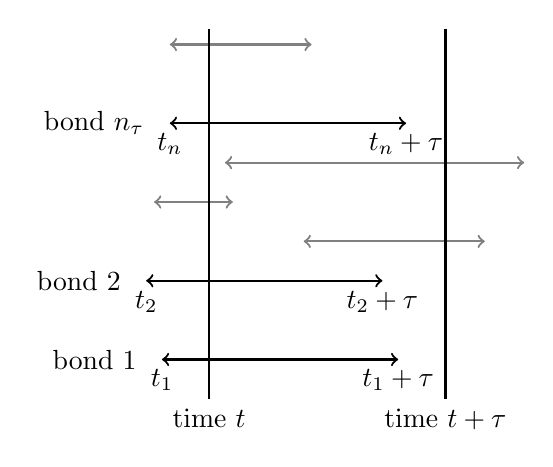
\begin{tikzpicture}[help lines/.style={thin,draw=black!50}]
%%\draw[help lines] (0,0) grid (4,4);
\draw [<->, thick] (0.4,0) node [anchor = north] {$t_1$} -- (3.4,0) node [anchor = north] {$t_1 + \tau$};
\draw (0.2,0) node [anchor = east] {bond $1$};
\draw [<->, thick] (0.2,1) node [anchor = north] {$t_2$} -- (3.2,1) node [anchor = north] {$t_2 + \tau$};
\draw (0,1) node [anchor = east] {bond $2$};
\draw [<->, thick] (0.5,3) node [anchor = north] {$t_n $} -- (3.5,3) node [anchor = north] {$t_n + \tau$};
\draw (0.3,3) node [anchor = east] {bond $n_{\tau}$};
\draw [gray,<->, thick] (1.2,2.5) -- (5.0,2.5);
\draw [gray,<->, thick] (0.3,2) -- (1.3,2);
\draw [gray,<->, thick] (2.2,1.5) -- (4.5,1.5);
\draw [gray,<->, thick] (0.5,4) -- (2.3,4) ;
\draw [thick] (1.0,4.2) -- (1.0,-0.5) node [anchor = north] {time $t$};
\draw [thick] (4.0,4.2) -- (4.0,-0.5) node [anchor = north] {time $t+\tau$};
\end{tikzpicture}
  \caption{\label{fig:P_tc} The H-bonds with lifetime $\tau$ in a certain configuration. 
At time $t$, we assume that there are totally $n_{tot}$ H-bonds can be detected, and $n_{\tau}$ H-bonds are of lifetime $\tau$, therefore,  the fraction of H-bonds that 
have the lifetime $\tau$ in the configuration at time $t$ is $P_{tc}(\tau) =  n_{\tau} /n_{tot}$.
Let $\tau$ take all the values in the interval $[0,\infty]$, we can get the HB lifetime distribution $P_{tc}(t)$.
}
\end{figure}
%\paragraph{Relation Between HB Dynamics and Anisotropy Decay}
%It is interesting to relate the HB kinetics with rotational dynamics (anisotropy decay) of single water molecules.\cite{HX01}
%
%\paragraph{Mean First Passage Time Probability Densities}

\paragraph{$k$ and $k'$: Least Squares Fit}
% TODO
%In order to show the effect of water molecule diffusion on the HB dynamics, we can calculate the sum of the functions $c(t)$ and $n(t)$, i.e., $c(t)+n(t)$.
The probability at time $t$ that a pair of water molecules bonded by H-bonds at the initial moment does not be bonded 
but the distance between their oxygen atoms is still less than $R_{OO}^c$ is 
\begin{eqnarray}
n(t) = \int_0^t dt'k_{in}(t'),
\label{eq:n_from_k_in}
\end{eqnarray}
where $k_{in}(t) = -\langle \dot h(0)[1-h(t)]h^d(t) \rangle/\langle h\rangle$ is the restricted rate function. 
Fig. \ref{fig:128w_bk_itp_50ps_n_from_k_in_with_2_hb_def}(a) and Fig.\ref{fig:128w_bk_itp_50ps_n_from_k_in_with_2_hb_def}(b)
show the function $n(t)$ in Eq. \ref{eq:n_from_k_in} for bulk water and water/vapor interface, respectively. 
In each figure, we have drawn the $n(t)$ function corresponding to the two different HB definitions. 
It can be found that the overall trend of n(t) does not depend on the choice of HB definition.
i.e., as $t$ increases, $n(t)$ increases rapidly from 0, and it reaches a maximum value at $t \approx 10$ ps, and then gradually decreases. %[EXPLAIN THE RESULTs]
Comparing the two figures \ref{fig:128w_bk_itp_50ps_n_from_k_in_with_2_hb_def}(a) and \ref{fig:128w_bk_itp_50ps_n_from_k_in_with_2_hb_def}(b),
we find that the maximum value of $n(t)$ in the water/vapor interface is slightly higher than that in bulk water. 
This feature does not depend on the definitions of the HB we choose.
%
\begin{figure}[H]
\centering
\includegraphics [width=0.6\textwidth] {./diagrams/128w_bk_itp_50ps_n_from_k_in_with_2_hb_def}
\setlength{\abovecaptionskip}{0pt}
\caption{\label{fig:128w_bk_itp_50ps_n_from_k_in_with_2_hb_def} 
The time dependence of the population functions $n(t)$ for (a) bulk water and (b) water/vapor interface, as computed from the ADH (solid line) and AHD (dashed line) 
criterion of H-bonds with the expression $n(t) = \int_0^t dt'k_{in}(t')$.} 
\end{figure}

Khaliullin and K\"uhne have studied the H-bonding kinetics of pure water using AIMD simulations. [\cite{Khaliullin2013}]
Based on the concepts of $h(t)$, $h^{(d)}(t)$, $n(t)$ and $k(t)$, they have used the simulation data 
obtained by the AIMD simulation method to obtain the ratio $k/k'$ in the bulk water, and then the lifetime and relaxation time 
of the HB.  Here, we also use the AIMD simulation method to study the HB dynamics at the interface of LiI, NaI, and KI aqueous 
solutions. We can obtain the optimal solution range of $k$ and $k'$ from the relationship 
between the reactive flux and the HB population correlation function $c(t)$ and $n(t)$, and the parameters $k$ and $k'$, i.e.,
\begin{eqnarray}
  k(t) = kc(t)-k'n(t).
\label{eq:fitting_k_rates}
\end{eqnarray}
%
%[Answer Q3]
We can find the optimal value of the parameters, $k$ and $k'$, 
by a least squares fit of the calculated data $k(t)$, $c(t)$ and $n(t)$ beyond the transition phase.  
The functions $c(t)$ can be regarded as a $P$-dimensional column vector composed by $(c(1),c(2),\cdots,c(P))^T$, and denoted as ${\bf c}$,
with $c(i)$ representing the value of the correlation $c(t)$ at $t=i$.
Similarly, the functions $n(t)$ and $k(t)$ can also be viewed as $P$-dimensional column vectors and can be denotd as ${\bf n}$ and ${\bf k}$, respectively.
Therefore, the $k$ and $k'$ can be determined from the matrix ${\bf A} = \begin{bmatrix} {\bf c} & {\bf n} \end{bmatrix}$, i.e., 
\begin{equation}
\begin{bmatrix} k\\ -k' \end{bmatrix} = ({\bf A}^T {\bf A})^{-1} A^T {\bf k}. 
\end{equation}
For bulk water and the water/vapor interface, the optimal $k$ and $k'$ are reported in Table 
\ref{tab:k_k_prime_128w_pure_1} and \ref{tab:k_k_prime_128w_pure_2}. 
% 
\begin{table}[htb]
\centering
\caption{\label{tab:k_k_prime_128w_pure_1} 
    The $k$ and $k'$ for the bulk water and the water/vapor interface. We carried on the short time region 0.2 ps $< t <$ 2 ps. 
The unit for $k$ ($k'$) is ps$^{-1}$, and that for $\tau_{\text{HB}}$ ($=1/k$) is ps.} 
\begin{tabular}{ccccccc}
 Criterion & $k$  (bulk) & $k'$ (bulk) & $\tau_{\text{HB}}$ (bulk) & $k$  (interf.) & $k'$ (interf.) & $\tau_{\text{HB}}$ (interf.)\\
\hline
  ADH & 0.3345 & 0.8591 & 2.9895 & 0.3587 & 0.6730 & 2.7881  \\
  ADH(from $k_{in}$) & 0.2959  & 0.9883 & 3.3795  & 0.3225 & 0.7652 & 3.1012 \\
  AHD & 0.3334 & 1.0414 & 2.9991 & 0.3520  & 0.7847  &  2.8405\\
  AHD(from $k_{in}$) & 0.2882 & 1.1490 & 3.4699 & 0.3140 & 0.8867 & 3.1836 \\
\end{tabular}
\end{table}
%
\begin{table}[htb]
\centering
\caption{\label{tab:k_k_prime_128w_pure_2} 
    The $k$ and $k'$ for the bulk water and the water/vapor interface. We carried on the long time region 2 ps $< t <$ 12 ps. 
The unit for $k$ ($k'$) is ps$^{-1}$, and that for $\tau_{\text{HB}}$ ($=1/k$) is ps.} 
\begin{tabular}{ccccccc}
 Criterion & $k$  (bulk) & $k'$ (bulk) & $\tau_{\text{HB}}$ (bulk) & $k$  (interf.) & $k'$ (interf.) & $\tau_{\text{HB}}$ (interf.)\\
\hline
  ADH & 0.1151 & 0.0311 & 8.6872 & 0.1593 & 0.0580 & 6.2786 \\
  ADH(from $k_{in}$) & 0.1147  & 0.0391 & 8.7184 & 0.1569  & 0.0678 & 6.3723\\
  AHD & 0.1071 & 0.0424 & 9.3450  & 0.1572 & 0.0763 & 6.3626 \\
  AHD(from $k_{in}$) & 0.1053  & 0.0472 & 9.4963 & 0.1545  & 0.0884 & 6.4715 \\
\end{tabular}
\end{table}
%
In the Table \ref{tab:k_k_prime_128w_pure_1} and \ref{tab:k_k_prime_128w_pure_2}, 
we performed the fitting in different time region $0.2 < t < 2$ ps and $2 < t < 12$ ps, respectively.
to obtain the forward and backward rate constants ($k$ and $k'$).
We note that in the larger time region, i.e., $2 < t < 12$ ps, the value of $\tau_R$ is larger than that in shorter time region, $0.2 < t < 2$ ps,
no matter for the bulk water or for the interface. A larger $\tau$ value means that the distance between a water molecule and another water molecule 
stays within $r_{OO}^c= 3.5$ \AA for a longer time. 
For the long time region, these values of the $k$ are comparable in magnitude to that obtained by Ref.\thinspace[{\cite{Khaliullin2013}}] 

%For AHD definition:The bulk water: 14.1572 ps; the water/vapor iterface: 12.7806 ps.


%For the water/vapor interface of pure water, we also calculated the constants $k$ and $k'$ by least square fit. 

\paragraph{LiNO$_3$ Solution} 
For a given molecular configuration, $\{\mathbf{r}_i (t)\}$, Eq. \ref{eq:rho_c} can be
solved through interpolation on a spatial grid.\cite{Willard2010} 
Figure \ref{fig:lino3_interface_all_add_z_trimed}
illustrates the obtained instantaneous interfaces for one configuration of a slab of 
LiNO$_3$ solution at 300 K.  We have taken $\{\mathbf{r}_i (t)\}$ to refer to the positions of all
atoms except hydrogen atoms in the system, and because the bulk correlation length of
liquid water is about one molecular diameter, we have used $\xi$ 
=2.4 \AA; further, we have used $\rho_0= 0.016$ \AA $^{-3}$, which is
approximately one-half the bulk density of water. 
\begin{figure}[H]
\centering
\includegraphics [width=0.32\textwidth] {./diagrams/lino3_interface_all_add_z_trimed}
\setlength{\abovecaptionskip}{0pt}
\caption{\label{fig:lino3_interface_all_add_z_trimed}
A slab of LiNO$_{3}$ solution with the instantaneous
interface $\mathbf{s}$ represented as a blue mesh on the upper and lower phase
boundary. The initial position of each ion in the solution is random.
The slab is periodically replicated in the horizontal directions.} 
\end{figure}
%

\begin{figure}[H]
\centering
\includegraphics [width=0.6\textwidth] {./diagrams/c_and_s_ln_bk_pbc}
\setlength{\abovecaptionskip}{0pt}
\caption{\label{fig:c_and_s_ln_bk_pbc} 
The time dependence of (a) $C_{HB}(t)$ and (b) ln$S_{HB}(t)$ of water--water and nitrate--water H-bonds at 300 K, 
as computed from the ADH (solid line) and AHD (dashed line) criterion of H-bonds. 
The definition of the correlation function is based on the specific HB configuration between molecules.} 
\end{figure}
The results of the correlation functions $C_{HB}(t)$ and $S_{HB}(t)$ for both nitrate--water (N--W) and water--water (W--W) H-bonds are shown in Fig. \ref{fig:c_and_s_ln_bk_pbc}(a) and (b), respectively.
For both HB definitions, it is found that the decay of the $C_{HB}(t)$ and $S_{HB}(t)$ for nitrate--water H-bonds is much faster 
than that for water--water H-bonds. From the relation \ref{eq:calculate_hb_lifetime_from_s}, the faster relaxation of $S_{HB}(t)$ implies that 
the nitrate--water H-bonds have shorter lifetime than the water--water H-bonds in the bulk phase. 
This result is obtained from a DFTMD simulation of a bulk phase of LiNO$_3$ solution at 300 K. The simulated system consisted of 127 water molecules and a Li$^+$--NO$_3^-$ ion pair
in a periodic cubic box of length $L=15.7787$\AA, which corresponds to a density of 1.11 g cm$^{-3}$. (TO CHECK) 

%
\section{Water-water Pair Based Hydrogen Bond Dynamics}
The method described in this paragraph is used more in the literature. 
The basis is the population operator $h(t)$ of the HB formed between two water molecules. 
We use the correlation function \CHB to describe the relaxation of H-bonds between two water molecules: [\cite{Luzar1994,AL96,AC00}]
\begin{eqnarray}
C_{\text{HB}}(t)=\langle h(0)h(t) \rangle/\langle h\rangle
\label{eq:C_HB}.
\end{eqnarray}
Similarly, with the aid of the ergodic principle, the ensemble average $\langle \cdots\rangle$ is implemented by time average.
The $\langle h\rangle$ is the probability that a pair of randomly chosen water molecules in the system is
H-bonded at any time $t$. 

The function \CHB is interpreted as the probability that the HB between a certain pair of water molecules is intact at time  $t$, 
if the pair of water molecules are H-bonded at time zero. 
In a large system that consist of many water molecules, the probability that a specific pair of water molecules are H-bonded is extremely small. 
Therefore, the \CHB relaxes to zero, when $t$ is large enough. 
The \CHB measures correlation in $h(t)$ independent of any possible bond breaking events. 
It is one of the intermittent HB correlation functions, introduced by Rapaport, [\cite{Rapaport1983}] 
and can be studied by a continuous function, probability densities.
From the \CHB, the HB relaxation time is computed as [\cite{Lee2007}]

Fig.\ref{fig:128w_bk_2delta_t_60ps_water_pair_c_ns40} shows the correlation function $C_{HB}(t)$ 
for bulk water over time. The result is calculated by DFTMD simulation, and the temperature is 300 K. 
\begin{figure}[H]
\centering
\includegraphics [width=0.360\textwidth] {./diagrams/128w_bk_2delta_t_60ps_water_pair_c_ns40}
\setlength{\abovecaptionskip}{0pt}
\caption{\label{fig:128w_bk_2delta_t_60ps_water_pair_c_ns40} 
The correlation functions $C_{HB}(t)$ for bulk water, based on water-water pair HB population operator $h(t)$, 
as computed from the ADH (solid line) and AHD (dashed line) criterion of H-bonds.} %[DESCRIBE THE FIGURE][COMPARE THE RESULTs TO hbond-based CORRELATION FUNCTION]
\end{figure}

% One can uncomment if remove PERCENT
%====================================
%Based on the HB definition of water molecule pairs, we can also use least squares fitting to obtain the rate constant $k$, $k'$, 
%and the average lifetime $\tau_{HB}$ of the H-bonds. The results are shown in the Table \ref{tab:k_k_prime_128w_pure_2s}  to \ref{tab:k_k_prime_128w_pure_2u}.
%\begin{table}[htb]
%\centering
%\caption{\label{tab:k_k_prime_128w_pure_2s} 
%    The $k$ and $k'$ for the bulk water and the water/vapor interface. We carried on the long time region 0.2 ps $< t <$ 8 ps. 
%The unit for $k$ ($k'$) is ps$^{-1}$, and that for $\tau_{\text{HB}}$ ($=1/k$) is ps.} 
%\begin{tabular}{ccccccc}
% Criterion & $k$  (bulk) & $k'$ (bulk) & $\tau_{\text{HB}}$ (bulk) & $k$  (interf.) & $k'$ (interf.) & $\tau_{\text{HB}}$ (interf.)\\
%\hline
%  ADH & 0.14 & 0.28 & 7.16 & - & - & -  \\
%  AHD & 0.11 & 0.18 & 9.08 & - & -  &  -\\
%\end{tabular}
%\end{table}
%%
%\begin{table}[htb]
%\centering
%\caption{\label{tab:k_k_prime_128w_pure_2t} 
%    The $k$ and $k'$ for the bulk water and the water/vapor interface. We carried on the longer time region 0.2 ps $< t <$ 12 ps. 
%The unit for $k$ ($k'$) is ps$^{-1}$, and that for $\tau_{\text{HB}}$ ($=1/k$) is ps.} 
%\begin{tabular}{ccccccc}
% Criterion & $k$  (bulk) & $k'$ (bulk) & $\tau_{\text{HB}}$ (bulk) & $k$  (interf.) & $k'$ (interf.) & $\tau_{\text{HB}}$ (interf.)\\
%\hline
%  ADH & 0.10 & 0.17 & 9.59 & - & - & -  \\
%  AHD & 0.09 & 0.11 & 11.62 & - & -  &  -\\
%\end{tabular}
%\end{table}
%%
%\begin{table}[htb]
%\centering
%\caption{\label{tab:k_k_prime_128w_pure_2u} 
%    The $k$ and $k'$ for the bulk water and the water/vapor interface. We carried on the longer time region 1 ps $< t <$ 12 ps. 
%The unit for $k$ ($k'$) is ps$^{-1}$, and that for $\tau_{\text{HB}}$ ($=1/k$) is ps.} 
%\begin{tabular}{ccccccc}
% Criterion & $k$  (bulk) & $k'$ (bulk) & $\tau_{\text{HB}}$ (bulk) & $k$  (interf.) & $k'$ (interf.) & $\tau_{\text{HB}}$ (interf.)\\
%\hline
%  ADH & 0.06 & 0.06 & 17.96  & - & - & -  \\
%  AHD & 0.06 & 0.05 & 18.17 & - & -  & -\\
%\end{tabular}
%\end{table}

\section{Interfacial Hydrogen Bond Dynamics}
\paragraph{Instantaneous interfaces}
As Willard and Chandler mentioned: "Due to molecular motions, interfacial configurations
change with time, and the identity of molecules that lie at the interface also change with time. Generally useful procedures for
identifying interfaces must accommodate these motions." \cite{Willard2010} 
To determine the instantaneous interface of the water/vapor system, we here adopted their proposed method based on spatial density.\cite{Willard2010}
The instantaneous coarse-grained density field at space-time point $\mathbf{r},t$ is given by 
\begin{eqnarray}
\bar{\rho}(\mathbf{r}, t)=\sum_{i} \phi(|\mathbf{r}-\mathbf{r}_{i}(t)|; \xi) 
\end{eqnarray}
where ${\mathbf{r}}_i$ is the position of the $i$th particle at time t and the sum is over all such particles, and 
\begin{eqnarray}
\phi(\mathbf{r};\xi)=(2 \pi \xi^{2})^{-3/ 2} \exp (-r^{2} / 2 \xi^{2}) \nonumber
\end{eqnarray} 
is a normalized Gaussian functions for a 3-dimensional system, where $\xi$ is the coarse-graining length.
With the parameter $\xi$ set, the interfaces can be defined to be the 2-dimensional manifold ${\mathbf r} = {\mathbf s}$ such that
\begin{eqnarray}
\bar\rho(\mathbf{s};t)= \rho_c 
\label{eq:rho_c}
\end{eqnarray} 
where $\rho_c$ is a reference density. This instantaneous interface is a function of time as molecular configurations changes with time, that is 
${\mathbf s}(t) = {\mathbf s}(\{{\mathbf r}_i(t)\})$. 

\paragraph{Instantaneous Layering of the water/vapor interface}
Once the instantaneous interface is defined, we can define an interface layer for any non-uniform fluid system. 
Specifically, for the water/vapor interface system we simulated in the cuboid simulation box, 
we can get another two-dimensional manifold ${\mathbf s}_0(t)$ by moving the instantaneous surface ${\mathbf s}(t)$ determined above 
along the system's normal coordinate to a certain distance $d$, which is another surface. We use these two surfaces 
as the two boundaries of the interface we will study. In other words, at any time point $t$, the volume between the two surfaces 
${\mathbf s}(t)$ and ${\mathbf s}_0(t)$ is defined as the instantaneous interface. 
Here, we call $d$ the thickness of the instantaneous interface. As long as we change the value of $d$, we can get interfaces with different thicknesses. 
Different values of $d$ give us different layering strategies for the interface system.

Below we will combine the instantaneous interface and Luzar-Chandler's HB population operator \cite{AL96} to select the H-bonds 
in the interface. The dynamics of these H-bonds will vary with the thickness $d$ of the interface. By investigating the characteristics of HB dynamics
in these interfaces, we can obtain the dynamical characteristics of various solution interfaces. As we will see later, this method can be extended to HB dynamics 
in various environments, such as H-bonds around certain ions, in bulk water, etc., so that we can more easily select H-bonds in a certain environment. 
These different environments have a common feature: because the molecular configuration changes over time, the usual method first selects these molecules or molecular pairs, 
and then determines the hydrogen bond in this special environment based on a HB criterion, and finally calculate the HB lifetimes or autocorrelation functions of 
the HB population operators. And here we are combining the general Luzar-Chandler HB population operator with the environment in which the HB is formed,
 that is, the space constraint satisfied by the configuration of the molecular pair. This combination can easily select those molecules and their H-bonds that meet arbitrary 
constraints when the molecular configuration changes.

\paragraph{Interfacial Hydrogen Bond}
Once we have determined the instantaneous surface ${\mathbf s}(t)={\mathbf s}(\{{\mathbf r}_i(t)\})$, we can define interface H-bonds.
We need one parameter $d$ to define the thickness of the instantaneous interface.
Now we can write the interface HB population operator $h^{s}[{\mathbf r}(t)]$ as follows:
It has a value 1 when the particular tagged molecular pair are bonded and both molecules are inside the instantaneous interface,
and zero otherwise.

Similar to the correlation function $C_{HB}(t)$ in Eq. \ref{eq:C_HB}, which describes the fluctuation of the general H-bonds,
 we can define the correlation function $C^s_{HB}(t)$ that describes the fluctuation of the interface H-bonds: 
\begin{eqnarray}
C^s_{\text{HB}}(t)=\langle h^s(0)h^s(t) \rangle/\langle h^s\rangle
\label{eq:C_s_HB}.
\end{eqnarray}
%
Based on the function $C^s_{HB}(t)$, we can define a similar correlation functions $k^s(t)$, $n^s_{HB}(t)$, $S^s_{HB}(t)$.
Therefore, using these new correlation functions, we can study the dynamics of interface hydrogen bonding.
%
\paragraph{$C^s_\text{HB}(t)$ as function of $d$}
\begin{figure}[htb]
\centering
\includegraphics [width=0.60\textwidth] {./diagrams/128w_itp_pure_water_pair_c_ihb}
\setlength{\abovecaptionskip}{0pt}
\caption{\label{fig:128w_itp_pure_water_pair_c_ihb} 
The correlation functions $C^s_{HB}(t)$ for the instantaneous interfacial H-bonds, based on water-water pair HB population operator $h^{s}(t)$, 
as computed from the (a) ADH and (b) AHD criterions of H-bonds.} 
\end{figure}
For the pure water interface, we used two geometric criteria for defining H-bonds to calculate the correlation function $C^s_{HB}(t)$. 
The calculation results are shown in Fig. \ref{fig:128w_itp_pure_water_pair_c_ihb}.
We can find that the greater the thickness of the interface is selected, 
the slower the relaxation of the interface H-bonds. When the thickness of the interface is greater than a critical thickness $d^c$ ( $\sim$ 5 \AA),
the relaxation of H-bonds at the interface hardly changes.

For comparison, let us look at the HB dynamics of water molecules in the interface obtained by selecting molecules 
located in instantaneous interface. (See Appendix \ref{ihb_and_selection}) 
The characteristic of this algorithm is to first select the molecules in the interface at each moment and make a statistical average of the correlation functions.
Specifically, in order to determine which water molecules are located in the interface, we sample at regular intervals, and then calculate 
the correlation function $C_{HB}(t)$ for the water molecules located in the interface and do a statistical average.
As the thickness of the instantaneous interface changes, the auto-correlation function of H-bonds in the interface we get will also change. 
Figure \ref{fig:128w_itp_pure_water_pair_c_ihb_scheme1} shows how the function $C_{HB}(t)$ changes with the thickness of the interface.
The sub-figure (a) and (b) use HB definition cirterion 1, and 2, respectively.
Comparing Fig. \ref{fig:128w_itp_pure_water_pair_c_ihb} and Fig. \ref{fig:128w_itp_pure_water_pair_c_ihb_scheme1}, we can see that
when we use the method of selecting molecules in the interface to calculate, the dependence of the correlation function $C_{HB}(t)$ ($C^s_{HB}(t)$) 
on the interface thickness is very consistent with the results obtained by the above-mentioned method . Moreover, regardless of the AHD definition 
or the ADH definition of the HB, this conclusion is valid. Since we want to study the HB dynamics in the interface, 
not just the correlation functions $C_{HB}(t)$ or $C^s_{HB}(t)$ in the interface, we will further examine the correlation functions $C_{HB}(t)$ ($C^s_{HB}(t)$), 
$n_{HB}(t)$, $k(t)$, and the rate constants $k$, $k'$ determined by these correlation functions.
\begin{figure}[H]
\centering                                         
\includegraphics [width=0.6\textwidth] {./diagrams/128w_itp_pure_water_pair_c_ihb_scheme1}
\setlength{\abovecaptionskip}{0pt}
\caption{\label{fig:128w_itp_pure_water_pair_c_ihb_scheme1} 
The correlation functions $C_{HB}(t)$ for the instantaneous interfacial H-bonds, based on water-water pair HB population operator $h(t)$, 
as computed from the (a) ADH and (b) AHD criterions of H-bonds. These results are based on selecting the water molecules in the interface and then averaging the 
HB dynamics of these water molecules. Sampling is performed every 4 ps. } 
\end{figure}

%[Plot the $k$ and $k'$ as functions of thickness $d$.]
\paragraph{Rate Constants $k$ and $k'$}  Figure \ref{fig:128w_itp_pure_water_pair_k_k_prime_ihb_both_schemes} compares the rate constants ($k$ and $k'$) 
and the lifetime $\tau_{HB}$ obtained by the two different methods mentioned above, i.e., IHB and molecule selection methods. 
We can see that, whether it is $k$, $k'$ or $\tau_{HB}$, their changing trend with the thickness of the 
interface is only slightly affected by the calculation method we use.
To illustrate this point more clearly, we compare the $k$, $k'$ and $\tau_{HB}$ obtained under the two methods.
%
\begin{figure}[H]
\centering
\includegraphics [width=0.6\textwidth] {./diagrams/128w_itp_pure_water_pair_k_k_prime_ihb_both_schemes}
\setlength{\abovecaptionskip}{0pt}
\caption{\label{fig:128w_itp_pure_water_pair_k_k_prime_ihb_both_schemes} 
The dependence of (a) the rate constants $k$ and $k'$ and (b) the lifetime $\tau_{HB}$ on the interface thickness,
obtained by the Instantaneous interface Hydrogen Bond (IHB) and by selecting the water molecules in the interface, respectively.
The corresponding $k$, $k'$ and $\tau_{HB}$ in the bulk water are also drawn with dashed lines as a reference.
(The $k$ of bulk water is represented by a black dashed line, and its $k'$ is represented by a blue dashed line.)
The constants are calculated based on the ADH criterion of H-bonds and the least square fits are carried on the time 
region 0.2 ps $< t <$ 12 ps.}
\end{figure}
We can see from Fig. \ref{fig:128w_itp_pure_water_pair_k_k_prime_ihb_both_schemes} that no matter which method is used, 
the trend of $k$ and $k'$ with the interface thickness is the same. 
Moreover, when the thickness is large enough ( $d \sim 5$ \AA ), these two constants agree well quantitatively. 
This very good result shows that the two extreme statistical methods used to calculate the HB dynamics of the interface did not produce 
much difference for the time scale (10$^2$ ps) and the scale ( 10$^2$ \AA ) of the simulation box we currently use.

We also found that when we look at the molecules in the interface whose thickness is less than 3 \AA, the values of the rate constants depend on the method we use. 
That is, the $k$ obtained by using the IHB method is relatively larger than the molecule selection method, and $k'$ is relatively smaller. 
At the same time, since $\tau_{HB} = 1/k$, this directly leads to a relatively shorter HB lifetime using the IHB method. 
This is related to our definition of IHB, and it is the same as our expectations: The definition of interface H-bonds makes the HB break rate 
on the interface artificially increased. At the same time, we know that the molecule selection method retains the original rate constant of H-bonds, 
but it may include the contribution of bulk water molecules to the rate constant. Therefore, the molecule selection method will underestimate the $k$. 

In Fig. \ref{fig:128w_itp_pure_water_pair_k_k_prime_ihb_both_schemes}, the $k$, $k'$ and $\tau_{HB}$ for the \emph{bulk} water are also drawn with dashed lines as a reference.
Comparing the above-mentioned physical quantities in the pure water interface and bulk water, we found that when the interface thickness is large enough, 
no matter which statistical method is used, the value of the reaction rate constants of the interface water we get is \emph{greater} than that in the bulk water. 
Therefore, since the HB lifetime can be calculated by $\tau_{HB} = 1/k$, the value of $\tau_{HB}$ in interface water is smaller than that in bulk water.

The more realistic HB dynamical properties of interface molecules are between the results of the above two methods. 
Therefore, it is possible to approximate the true appearance of the HB dynamics of the interface molecules, 
by both the IHB method and the molecule selection method if the thickness of the interface is selected large enough. 

In summary, if we study the dynamics of H-bonds in a very thin interface, we can use the method of molecular selection, 
because the H-bonds obtained in this way are not artificially broken, and if the interface we study is thick enough, for example, if it is greater than 3 \AA
(see Fig. \ref{fig:128w_itp_pure_water_pair_k_k_prime_ihb_both_schemes}a), then we can use the IHB method, because it can automatically define which H-bonds come 
from the interface without the need to select the water molecules in the interface layer.
%
\begin{table}[htb]
\centering
\caption{\label{tab:k_k_prime_tau_128w_pure_ihb_ADH} 
    The $k$ and $k'$ for the interfacial hydrogen dynamics of the water/vapor interface (by the method of IHB and of ADH criteria). 
We carried on the longer time region 0.2 ps $< t <$ 12 ps. The unit for $k$ ($k'$) is ps$^{-1}$, and for $\tau_{\text{HB}}$ ($=1/k$) 
is ps. The thickness $d$ (\AA) denotes the thickness of the interface, which is obtained from the instantaneous surface. 
The parameter values and units are the same below.} 
\begin{tabular}{cccc}
 Thickness & $k$ & $k'$ & $\tau_{\text{HB}} (=1/k)$ \\
\hline
  1.0 & 0.653 & 0.080 & 1.53  \\
  2.0 & 0.261 & 0.133 & 3.83  \\
  3.0 & 0.168 & 0.104 & 5.94  \\
  4.0 & 0.148 & 0.092 & 6.76  \\
  5.0 & 0.147 & 0.087 & 6.81  \\
  6.0 & 0.139 & 0.087 & 7.17  \\
\end{tabular}
\end{table}
\begin{table}[htb]
\centering
\caption{\label{tab:k_k_prime_tau_128w_pure_ihb_AHD} 
    The $k$ and $k'$ for the interfacial hydrogen dynamics of the water/vapor interface (by the method of IHB and of AHD criteria).} 
\begin{tabular}{cccc}
 Thickness & $k$ & $k'$ & $\tau_{\text{HB}} (=1/k)$ \\
\hline
  1.0 & 0.661 & 0.080 & 1.51  \\
  2.0 & 0.265 & 0.133 & 3.77  \\
  3.0 & 0.172 & 0.102 & 5.82  \\
  4.0 & 0.148 & 0.090 & 6.74  \\
  5.0 & 0.149 & 0.084 & 6.72  \\
  6.0 & 0.144 & 0.078 & 6.93  \\
\end{tabular}
\end{table}

\begin{table}[htb]
\centering
\caption{\label{tab:k_k_prime_tau_128w_pure_ihb_scheme1_ADH} 
    The $k$ and $k'$ for the interfacial hydrogen dynamics of the water/vapor interface (by the method of molecule selection and of ADH criteria).} 
\begin{tabular}{cccc}
 Thickness & $k$ & $k'$ & $\tau_{\text{HB}} (=1/k)$ \\
\hline
  1.0 & 0.526 & 0.072 & 1.90  \\
  2.0 & 0.246 & 0.158 & 4.07  \\
  3.0 & 0.160 & 0.114 & 6.26  \\
  4.0 & 0.140 & 0.097 & 7.15  \\
  5.0 & 0.138 & 0.090 & 7.24  \\
  6.0 & 0.125 & 0.080 & 8.00  \\
  7.0 & 0.133 & 0.085 & 7.49  \\
\end{tabular}
\end{table}
\begin{table}[htb]
\centering
\caption{\label{tab:k_k_prime_tau_128w_pure_ihb_AHD} 
    The $k$ and $k'$ for the interfacial hydrogen dynamics of the water/vapor interface (by the method of molecule selection and of AHD criteria).} 
\begin{tabular}{cccc}
 Thickness & $k$ & $k'$ & $\tau_{\text{HB}} (=1/k)$ \\
\hline
  1.0 & 0.610 & 0.083 & 1.64  \\
  2.0 & 0.235 & 0.142 & 4.62  \\
  3.0 & 0.138 & 0.102 & 7.22  \\
  4.0 & 0.141 & 0.098 & 7.07  \\
  5.0 & 0.120 & 0.078 & 8.40  \\
  6.0 & 0.117 & 0.072 & 8.58  \\
  7.0 & 0.119 & 0.071 & 8.39  \\
\end{tabular}
\end{table}

%===============================================
\section{Interface of Lithium Nitrate Solutions}
%===============================================
For the molecular dynamics trajectory of a solution interface, we can now get instantaneous surface.
For any molecule or ion $\alpha$ in such a solution interface system, we can get its distance from the lower and upper instantaneous surfaces.
We assume that the $z$-axis is the normal direction, then the distances between the particle and the two instantaneous surfaces are:
%
\begin{eqnarray}
    d_{\alpha,1}(t)= z_{\alpha}(t) - z^{surf}_{\alpha,1}(t),  \\
    d_{\alpha,2}(t)= z^{surf}_{\alpha,2}(t) - z_{\alpha}(t), 
\label{eq:distance_particle2surf}
\end{eqnarray}
%
where $z_{\alpha}(t)$ is the coordinate of the particle $\alpha$ in the normal direction at time $t$, 
$z^{surf}_{\alpha,i}(t)$ is the $z$ coordinate of the surface position corresponding to particle $\alpha$ at time $t$, 
and the subscripts $i=1$ and 2 respectively identify the lower and upper instantaneous surfaces.
As an example, Fig. \ref{fig:lino3_interface_ions_add_z_and_d_and_label_2_trimed} shows the distances, 
$d_{\text{Li}^+,1}$ and $d_{\text{NO}_3^-,1}$, between ions and one of the instantaneous surfaces at a certain moment.
%
\begin{figure}[H]
\centering
\includegraphics [width=0.32\textwidth] {./diagrams/lino3_interface_ions_add_z_and_d_and_label_2_trimed}
\setlength{\abovecaptionskip}{0pt}
\caption{\label{fig:lino3_interface_ions_add_z_and_d_and_label_2_trimed}
The distances between ions and one of the instantaneous surface for a slab of aqueous LiNO$_3$ solution.}
\end{figure}


Figure \ref{fig:dist_li_surf_lino3_interface} shows the time dependence of the distance between the anion (cation) 
and the two instantanous surfaces in the LiNO$_3$ solution at 300 K. We found that when the system reaches an equilibrium state, 
the lithium ions are stably within a few angstroms below the interface, while the nitrate ion are more willing to be on the surface. 
When the system is in equilibrium ($t>10$ ps), the distance $d_{NO_3^-,1}$ is even sometimes \emph{negative}. 
This negative distance strongly proves from the first-principles calculation that nitrate ions are more willing to be on the interface. 
Therefore, the results calculated using the instantaneous interface are consistent with the results of the SFG spectra of the LiNO$_3$ solution.
%
\begin{figure}[htbp]
\centering
\includegraphics [width=0.6 \textwidth] {./diagrams/dist_li_surf_lino3_interface} 
\setlength{\abovecaptionskip}{0pt}
  \caption{\label{fig:dist_li_surf_lino3_interface} Time dependence of the cation--surface and nitrate--surface distances at 300 K.}
\end{figure}
%
\paragraph{Experiments on HB Dynamics}
[TODO]
Experimentally Ref.  \cite{Radnai1995}
An important  structural characteristic of the H-bonded network is the average number of H-bonds per molecule, $\langle h_{i,j}\rangle$. \cite{Chowdhary2009} 
For bulk water systems, we find the average number of hydrogen bonds in the bulk phase is $\sim$ 4.35 which is slightly
(higher) than the usual estimate of 3.4 (interface system) for SPC/E water.

For interfacial systems of neat water, we find the average number
of hydrogen bonds is 3.XX which is slightly
(lower/higher) than the usual estimate of 3.4 for SPC/E water. \cite{Chowdhary2009}

%===============================================
\section{Rotational Anisotropy Decay of Water at the Interface of Alkali-Iodine Solutions}\label{CHAPETR_AD}
%===============================================
Using the transition dipole auto-correlation function, 
we determined the rotational anisotropy decay and therefore the OH-stretch relaxation at water/vapor interface of alkali iodide solutions.
%The effects of ion environment on structure and dynamics of water are obtained by comparing the second-order Legendre polynomial, i.e.,  $P_2(x)=\frac{1}{2}(3x^2-1)$,  orientational correlation function of the transition dipole.
The anisotropy decay can be determined from experimental signal in two different polarization configurations---parallel and perpendicular polarizations, by 
\begin{equation}
        R(t)=\frac{S_{\parallel}(t)-S_{\perp}(t)}{S_{\parallel}(t)+2S_{\perp}(t)}
\label{eq:ad}
\end{equation}
where $t$ is the time between pump and probe laser pulses.  The anisotropy decay can also be obtained by simulations, 
and calculated by the third-order response functions $R(t)$. [\cite{Jansen10,Jansen06}]
%
%In the first shell with a radius 3 \A, the entropy difference betweem the \Li shell and \Na shell,
%$\Delta S=k_B\text{ln}\frac{\Omega_\text{Na}}{\Omega_\text{Li}}=k_B\text{ln}\frac{n_\text{Na}/V_\text{Na}}{n_\text{Li}/V_\text{Li}} =k_B\text{ln}1.05$.
%
%\paragraph{Probability Distribution of Ions}
%The probability distribution, shown in Fig.~\ref{fig: prob_124_LiI_Sans_double_axis}, of the ions in the water/vapor interface of LiI and NaI solutions with repect to the depth of the ions in the solutions 
%indicates that the \I ions prefer to staying at the topmost layer of surface of solutions.
%(molar concentration: 0.9 M, temperature: 330 K) 
%It shows that \I ions tend to the surface of the solutions, while \Na and \Li tend to stay in the bulk. This result is consistent with the calculations from Ishiyama and Morita\cite{TI07,TI14}.
The orientational anisotropy $C_2(t)$ is given by the rotational time-correlation function 
\begin{equation}
C_2(t)=\langle P_2(\hat{u}(0)\cdot\hat{u}(t)) \rangle,
\label{eq:tcf2}
\end{equation}
where $\hat{u}(t)$ is the time dependent unit vector of the transition dipole, $P_2(x)$ is the second Legendre polynomial, and $\langle \cdots \rangle$ indicate 
equilibrium ensemble average. [\cite{Corcelli05,LinYS2010}] %\cite{2010Lin} % angular brackets

The anisotropy decay $C_2(t)$ for the water/vapor interface of LiI solution is shown in Fig.\space\ref{fig:c2_2LiI_16_inset}.
This function decays faster than that of neat water, indicating that H-bonds
at the interfaces of alkali-iodine solutions reorient faster than in neat water. The inset shows the first 0.4 ps of $C_2(t)$, from which we see a 
quick change during the first $\sim 0.1$ ps primarily due to librations.
%
\begin{figure}[h]
\centering
\includegraphics [width=0.36\textwidth] {./diagrams/c2_2LiI_16_inset} 
\setlength{\abovecaptionskip}{0pt}
  \caption{\label{fig:c2_2LiI_16_inset} The time dependence of the $C_2(t)$ of OH bonds at the water/vapor interfaces of 0.9 M LiI solution 
    and of neat water (dashed line) at 330 K, calculated by DFTMD simulations.} 
    %The water/vapor interface of neat water is modeled 
    %with a slab made of 121 water molecules in a simulation box of size $15.6 \times 15.6 \times 31.0$ \A$^3$.
\end{figure}
%
We also calculated the $C_2(t)$ for the interface of other alkali-iodine solutions LiI and KI. 
The results of $C_2(t)$ for the water/vapor interfaces of these solutions are shown in Fig.\space\ref{fig:c2_2KI_2NaI_2LiI_16}.
In all the cases $C_2(t)$ decays faster than in neat water, indicating that H-bonds
at the interfaces of the three alkali-iodine solutions are orientated faster than that of neat water.
They show that \I ions can accelerate the dynamics of molecular reorientation of water molecules at interfaces.   

%
\begin{figure}[htbp]
\centering
\includegraphics [width=0.36\textwidth] {./diagrams/c2_2KI_2NaI_2LiI_16} 
\setlength{\abovecaptionskip}{0pt}
  \caption{\label{fig:c2_2KI_2NaI_2LiI_16} The time dependence of the $C_2(t)$ of OH bonds in water molecules at the water/vapor 
  interface of 0.9 M alkali-iodine solutions and of neat water (dashed line) at 330 K, calculated by DFTMD simulations.}
\end{figure} 

We have obtained non-single-exponential kinetics for the rotation of water molecules both at the surface 
and in bulk water (Appendix \ref{single_exp}).
%This result is true for water molecules bound to ions. 
Therefore, the rotational motion of water molecules are not simply characterized by well-defined rate constants. 
%Then the problem is to understand the kinetics.
Similar non-single-exponential kinetics is also obtained in the HB kinetics
in liquid water [\cite{AL96,Dirama05}] and in the time variation of the average frequency shifts of the 
remaining modes after excitation in hole burning technique [\cite{Rey2002,Moller2004}] and using BLYP functional. [\cite{Bankura2014}]
Luzar and Chandler interpreted 
the non-single-exponential kinetics as the result of an interplay between 
diffusion and HB dynamics. [\cite{AL96}] 
We can understand the non-single-exponential kinetics of rotational 
anisotropy decay by fitting the rotational anisotropy decay by a 
biexponential function.

To obtain the effects of diffusion and HB decay of water molecules
in solutions respectively, we assume that there are two independent 
decays in the process of an anisotropy decay. 
Therefore, the $C_2(t)$ has the form [\cite{TanHS05}]
\begin{equation}
C_2(t)=A_1e^{-\kappa_1 t} +A_2e^{-\kappa_2 t},
\label{eq:tcf3}
\end{equation}
where $A_i$ are constants and $\kappa_i$ are decay rates ($i=1, 2$). 
The time constants and amplitudes of the biexponentials fits for 
the $C_2(t)$ are listed in Table ~\ref{tab:2LiI_c2_biexp} and Table ~\ref{tab:2NaI_c2_biexp}.
The biexponential fit is very close to the calculated $C_2(t)$, which can be seen in Fig.\space\ref{fig:2LiI-124w_c2_fit_5ps_biexp} (compare Fig.\space\ref{fig:2LiI-124w_c2_fit_5_single-exp}).
%
\begin{table}[hbt]
\centering
\caption{\label{tab:2LiI_c2_biexp}%
	Biexponential fitting (5 ps) of the $C_2(t)$ for water molecules in 0.9 M LiI solution.}
%\begin{ruledtabular}
\begin{tabular}{lccccc}
water molecules & $A_1$  & $\kappa_1$ (THz) & $A_2$ & $\kappa_2$ (THz) \\
\hline
I$^-$-shell & 0.44 & 0.25 & 0.39 & 0.26\\
Li$^+$-shell & 0.88 & 0.07 & 0.07 & 8.24\\
bulk & 0.84 & 0.11 & 0.09 & 4.88 \\
surface & 0.73 & 0.27 & 0.22 & 13.47 \\
\end{tabular}
%\end{ruledtabular}
\end{table}
%--

\begin{table}
\centering
  \caption{\label{tab:2NaI_c2_biexp}%
	Biexponential fitting (5 ps) of the $C_2(t)$ for water molecules in 0.9 M NaI solution.}
  \begin{tabular}{lccccc}
  water molecules & $A_1$  & $\kappa_1$ (THz) & $A_2$ & $\kappa_2$ (THz) \\
  \hline
  I$^-$-shell & 0.86 & 0.14 & 0.08 &9.86 \\
  Na$^+$-shell & 0.71 & 0.06 & 0.18 &0.79 \\
  bulk & 0.81 & 0.06 & 0.10 & 1.25 \\
  surface & 0.77 & 0.11 & 0.13 & 2.31 \\
  \end{tabular}
\end{table}
%
%图
\begin{figure}[htbp]
\centering
\includegraphics [width=0.60\textwidth] {./diagrams/2LiI-124w_c2_fit_5_biexp} 
  \caption{\label{fig:2LiI-124w_c2_fit_5ps_biexp} The time dependence of the $C_2(t)$ of OH bonds 
  in water molecules at the water/vapor interface of LiI solution.}
\end{figure} 
%
%[Notes: The 63-water-slab models is listed here as a reference. The number of water molecules is small; The data for KI/vapor and LiI/vapor interfaces come from  KI\_16 and LiI\_16 systems.  
%Water(63) &0.831$\pm(1\times10^{-4})$ &  0.08760 $\pm(2\times 10^{-5})$&0.100$\pm(2\times10^{-4})$ & 1.029 $\pm(4\times10^{-3})$  \\ ]
%
%\begin{figure}[htbp]
%\centering
%\includegraphics [width=0.4 \textwidth] {./diagrams/c2_121-pure_2KI_2LiI_16_inset_fit_biexp} 
%\setlength{\abovecaptionskip}{10pt}
%\caption{\label{fig:c2_121-pure_2KI_2LiI_16_inset_fit_biexp} The fitted and calculated anisotropy decay of OH bonds in water molecules in LiI solution/vapor interface (red), LiI solution/vapor interface (blue) and neat water/vapor interface (black). The corresponding fitted functions are denoted by dashed lines. The concentration of LiI and KI solution is 0.9 M.}
%\end{figure} 

Then we considered the effect of ion species in solutions on the anisotropy decay of water molecules.
From Table \ref{tab:2LiI_c2_biexp} and Table \ref{tab:2NaI_c2_biexp}, we find that 
for both LiI and NaI solutions, there are two decay processes in the dynamics --- amplitude $\sim 1$,
decay constant $\sim$ 0.1 THz, and for the other describe the initial fast decay 
of the anisotropy, with amplitude $\sim 0.1$, decay constant $\sim$ (1--10) THz, 
due to the inertial-librational motion preceding the orientational diffusion.
That is, two decay processes exist in the dynamics of water molecules 
at the water/vapor interfaces of alkali-iodine solutions. 
%The one describe the initial fast decay of the anisotropy, 
%with amplitude $\sim$ 0.1, decay constant $\sim$ (1--10) THz,
%results from the inertial-librational motion preceding the orientational diffusion.
%%
%\begin{table}[H]
%\centering
%\caption{\label{tab:fitting_c2_for_each_type_of_water}%
%  Biexponentially fitting (2 ps) of the $C_2(t)$ for different types of water molecules at the water/vapor interface of LiI solutions.}
%\begin{tabular}{lccccc}
%water molecules & $A_1$  & $\kappa_1$ (THz) & $A_2$ & $\kappa_2$ (THz) \\
%\hline
%$DDAA$ & 0.85 & 0.25   & 0.10 & 16.0\\
%$DD'AA$ & 0.89 & 0.14  & 0.06 & 14.1 \\
%$D'AA$ & 0.38 & 0.99 & 0.38 & 0.99 \\
%\end{tabular}
%\end{table}
%%
%\begin{table}[H] %[!hbtp]
%\centering
%\caption{\label{tab:table_CoordNo}%
%The coordination number of the atoms in LiI (NaI) solutions.}
%\begin{tabular}{lccc}
%name & radius of the first shell (\AA) & coordination number \\
%\hline
%$n_\text{I-H}(\text{LiI})$ & 3.3 & 5.5 \\
%$n_\text{I-H}(\text{NaI)}$ & 3.3 & 5.1 \\
%$n_\text{I-O}(\text{LiI)}$ & 4.3 & 5.8 \\
%$n_\text{I-O}(\text{NaI)}$ & 4.3 & 6.0 \\
%$n_\text{Li-O}(\text{LiI)}$ & 3.0 & 4.0 \\
%$n_\text{Na-O}(\text{NaI)}$ & 3.5 & 6.0 
%\end{tabular}
%\end{table}

\section{I$^-$--Water Hydrogen Bonds in Aqueous Solutions}
In the case of water--water H-bonds, the critical distance of $r_{OO}^c=3.5$ \AA are the position of the first minimum of the oxygen--oxygen RDF.
For the anion--oxygen H-bonds, we can use the similar criteria. The cutoff values for $X$--oxygen distance are obtained from the positions of the first
minimum of the $X$--oxygen RDF, i.e., $R_c^{XO}=4.1$, 3.7 \A, for $X$ = I$^-$ and nitrate O. We have still used $30^{\circ}$ for the anglar cutoff.\cite{Chowdhuri2006}
\begin{figure}[htbp]
\centering
\includegraphics [width=0.6 \textwidth] {./diagrams/gdr_127_LiNO3} 
\setlength{\abovecaptionskip}{0pt}
  \caption{\label{fig:gdr_127_LiNO3} (a)Li--water O, Li--water H RDFs; (b) Nitrate O--water O, nitrate O-water H RDFs for LiNO$_3$ solutions at 300 K. The RDFs were computed from DFTMD.}
\end{figure}
The function $C_{HB}$ of I$^-$--water and water--water H-bonds describes the structural relaxation of these H- bonds. The results of the $C_{HB}(t)$ are shown in Fig. \ref{fig:X-O_c_lii}. 
\begin{figure}[htbp]
\centering
\includegraphics [width=0.6 \textwidth] {./diagrams/X-O_c_lii} 
\setlength{\abovecaptionskip}{0pt}
  \caption{\label{fig:X-O_c_lii} Time dependence of the intermittent correlation functions of I$^-$--water (I$^-$--W) and water--water H-bonds at 300 K.}
\end{figure}
The results of the continuous correlation functions for both definitions (ADH and AHD criterions) for the H-bonds are shown in Fig. \ref{fig:wat-wat_s_lii} 
for I$^-$--water H-bonds. The results of water--water H-bonds are also included for comparison in both Fig. \ref{fig:wat-wat_s_lii} (a) and (b).
\begin{figure}[htbp]
\centering
\includegraphics [width=0.6 \textwidth] {./diagrams/wat-wat_s_lii} 
\setlength{\abovecaptionskip}{0pt}
  \caption{\label{fig:wat-wat_s_lii} Time dependence of the continuous correlation functions of I$^-$--water (I$^-$--W) and water--water H-bonds at 300 K.}
\end{figure}
For both definitions for the H-bonds, it is found that the I$^-$--water H-bonds show faster dynamics than water--water H-bonds. 
(consistent to the previous MD results.) Therefore, the time scales of the relaxation of these H-bonds can be obtained for both definitions. 
In Table \ref{tab:properties_anion-water_hbs}, we have included the average lifetimes $\langle\tau_{a}\rangle$ for both water--water and I$^-$--water H-bonds. 
We performing the fitting in the time region 0.2 ps < $t$ < 12 ps to calculate the forward and backward rate constants for HB breaking.
%
\begin{table}[htbp]
\centering
\caption{ 
    The Dynamical properties of anion--water and water--water H-bonds at 300 K. Data are from DFTMD for the aqueous solutions. The values are expressed in ps.} 
\begin{tabular}{ccccc}
\label{tab:properties_anion-water_hbs}
 Quantity & Criterion & W--W & I$^-$--W & NO$_3^-$--W  \\
\hline
  $\langle\tau_a\rangle$  & ADH & 190.3 & 0.10 & 4.35 \\
  $\langle\tau_a\rangle$ & AHD & 186.8  & 0.11 & 7.91 \\
  $1/k$ & ADH & 9.82 & 2.80 & 4.15 \\
  $1/k$ & AHD & 8.97 & 2.40 & 6.02\\
\end{tabular}
%
% Data from: LiI solution:  gang@XPS /home/gang/Github/water_pair_HB_dynamics/src/least_square_fit
% Data from: LiNO3 solution:  /home/gang/Github/water_pair_HB_dynamics/src/least_square_fit/LiNO3 
\end{table}
\begin{figure}[htbp]
\centering
\includegraphics [width=0.6 \textwidth] {./diagrams/I--wat_n_lii} 
\setlength{\abovecaptionskip}{0pt}
  \caption{\label{fig:I--wat_n_lii} Time dependence of the correlation functions $n_{HB}(t)$ of I$^-$--water (I$^-$--W) and water--water H-bonds at 300 K.}
\end{figure}

